\chapter{Proposta}

\section{Visão Geral}

O projeto consiste em uma plataforma de aprendizado de programação em Python, com foco em iniciantes. A plataforma será composta por um conjunto de quizzes, desafios e projetos, que serão utilizados para fixar o conteúdo aprendido. A plataforma também contará com um sistema de pontuação, que será utilizado para incentivar os usuários a realizarem os quizzes, desafios e projetos, além de compartilharem seus projetos com outros usuários. A plataforma também contará com um sistema de ranking, que será utilizado para mostrar aos usuários o desempenho deles em relação aos outros usuários.

\section{Especificação de Requisitos}

\subsection{Requisitos Funcionais}

Os requisitos funcionais do projeto são:

\begin{itemize}
    \item RF01: Cadastro de usuários: o sistema deve permitir que os usuários se cadastrem na plataforma.
    \item RF02: Login de usuários: o sistema deve permitir que os usuários façam login na plataforma.
    \item RF03: Visualização de quizzes e desafios: o sistema deve permitir que os usuários visualizem quizzes e desafios.
    \item RF04: Realização de quizzes: o sistema deve permitir que os usuários realizem quizzes para fixar o conteúdo.
    \item RF05: Realização de desafios: o sistema deve permitir que os usuários realizem desafios para fixar o conteúdo.
    \item RF06: Criação de projetos: o sistema deve permitir que os usuários criem projetos em Python.
    \item RF07: Compartilhamento de projetos: o sistema deve permitir que os usuários compartilhem projetos através de links.
    \item RF08: Pontuação: o sistema deve permitir que os usuários acumulem pontos ao realizar quizzes, desafios, projetos e compartilhar projetos.
    \item RF09: Visualização da pontuação: o sistema deve permitir que os usuários visualizem sua pontuação.
    \item RF09: Visualização de ranking: o sistema deve permitir que os usuários visualizem o ranking de pontos.
    \item RF10: Visualização do histórico de pontuação: o sistema deve permitir que os usuários visualizem o histórico de pontuação.
    \item RF11: Visualização do perfil: o sistema deve permitir que os usuários visualizem seu perfil.
    \item RF12: Edição do perfil: o sistema deve permitir que os usuários editem seu perfil.
    \item RF13: Exclusão do perfil e dados: o sistema deve permitir que os usuários excluam seu perfil e dados.
\end{itemize}

\subsection{Requisitos Não-Funcionais}

Os requisitos não-funcionais do projeto são:

\begin{itemize}
    \item RNF01: Login simples: o sistema deve permitir que os usuários façam login com apenas um clique.
    \item RNF02: Cadastro simples: o sistema deve permitir que os usuários se cadastrem com apenas um clique.
    \item RNF03: Disponibilidade: o sistema deve estar disponível 24 horas por dia, 7 dias por semana.
    \item RNF04: Segurança: o sistema deve ser seguro, com criptografia de dados e autenticação de usuários.
    \item RNF05: Usabilidade: o sistema deve ser fácil de usar, com uma interface simples e intuitiva.
    \item RNF06: Escalabilidade: o sistema deve ser escalável, podendo ser facilmente adaptado para suportar um número maior de usuários.
    \item RNF07: Portabilidade: o sistema deve ser inicialmente desenvolvido para rodar em navegadores web, mas deve ser facilmente adaptado para rodar em outros dispositivos.
    \item RNF08: Qualidade: o sistema deve ser de alta qualidade, com ferramentas de analise de código e testes automatizados.
\end{itemize}

\section{Protótipo de Alta Fidelidade}

% \begin{figure}[H]
%     \centering
%     \includegraphics[width=0.8\textwidth]{prototipo.eps}
%     \caption{Protótipo de Alta Fidelidade}
%     \label{fig:prototipo}
% \end{figure}

\section{Cronograma}

O cronograma foi dividido em 6 fases, sendo que cada fase possui um prazo de 2 semanas, sendo elas:

\begin{itemize}
    \item Fase 1: Reestruturação do trabalho existente; Levantamento de requisitos; criação do modelo de dados, arquitetura e pacotes.
    \item Fase 2, 3 e 4: Desenvolvimento do sistema.
    \item Fase 5: Correção de bugs e ajustes finais; Análise e coleta de resultados.
    \item Fase 6: Documentação e apresentação do projeto.
\end{itemize}

\subsection{Gráfico de Gantt}

\begin{figure}[H]
    \centering
    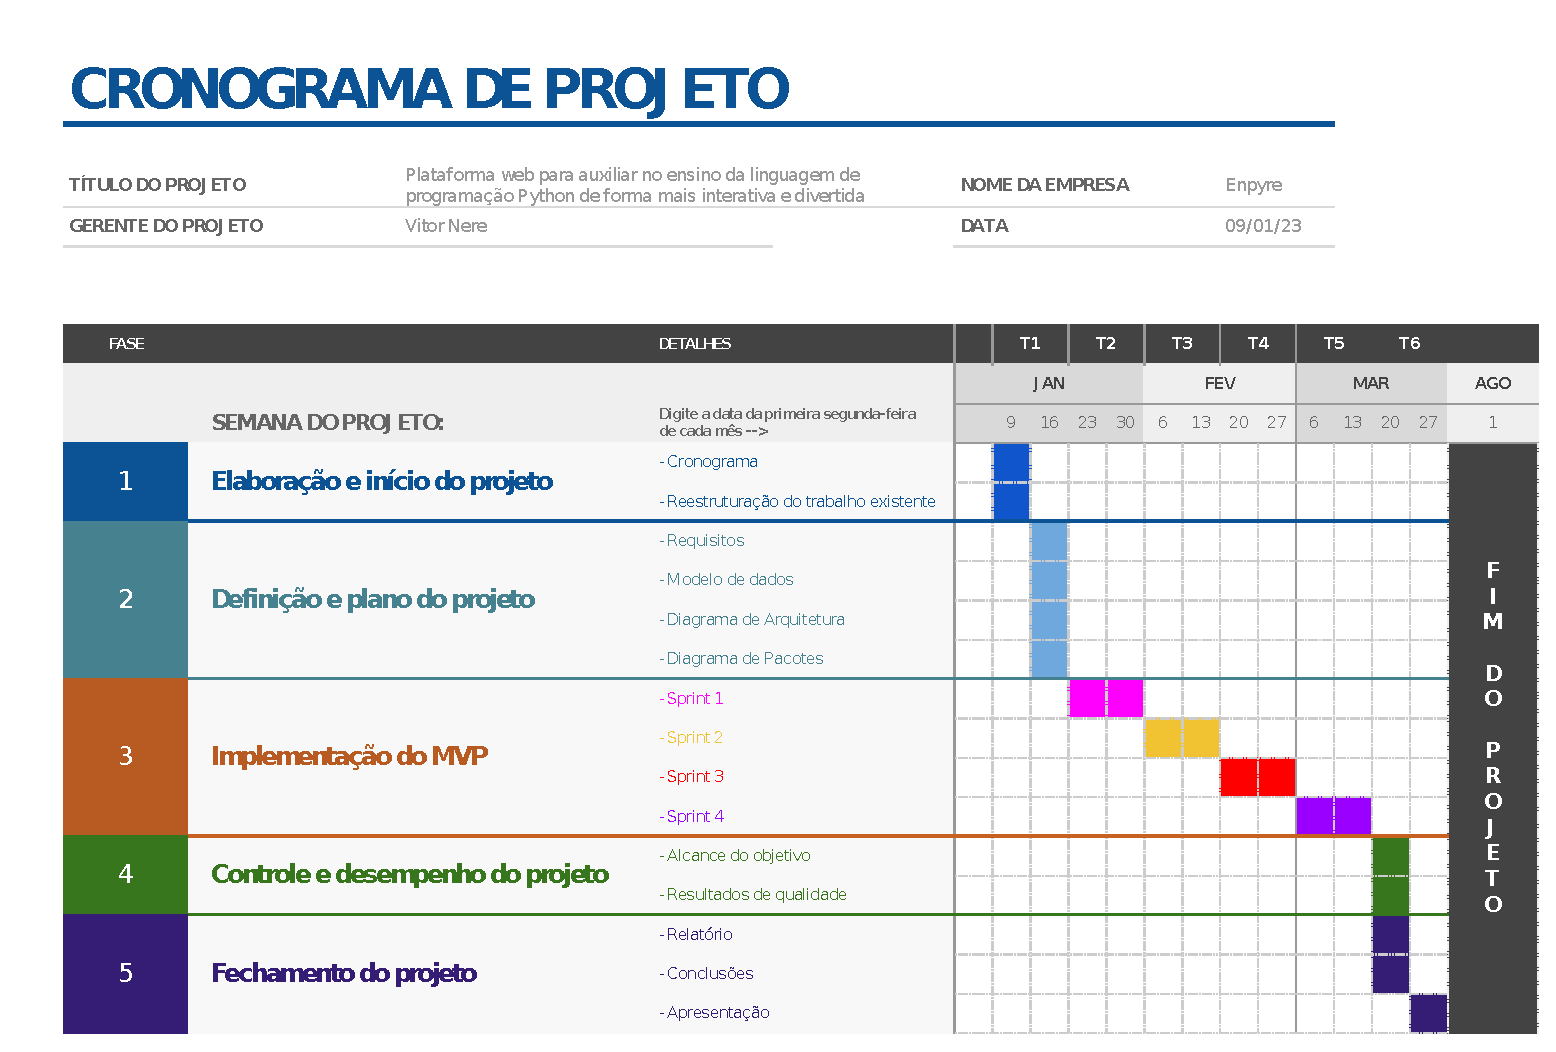
\includegraphics[width=1.1\textwidth]{figuras/cronograma.eps}
    \caption{Gráfico de Gantt}
    \label{fig:gantt}
\end{figure}
